\documentclass[]{report}
\usepackage{graphicx}
\usepackage{geometry}
\usepackage{amssymb}
\usepackage{textcomp}
 \geometry{
 a4paper,
 total={170mm,257mm},
 left=20mm,
 top=20mm,
 width=17cm,
 }
\usepackage{ragged2e}

\begin{document}
\begin{center}
 {\Large Data Intensive Computing - Review Questions 3}
\end{center}
\begin{center}
 {\small Daniele Montesi, Francesco Staccone}
\end{center}
\vspace{1cm}
\justify
\begin{enumerate}
 \item Briefly compare the DataFrame and DataSet in SparkSQL and via one example show when it is beneficial to use DataSet instead of DataFrame.\\
 
\noindent Both DataFrames and DataSets are structured collections used in Spark to work with data. They are immutable, that's why Spark performs lazy evaluations when working on them, returning always a new copy.

\begin{itemize}
    \item \textbf{DataFrames} have the idea to replace RDDs (functional transformation, collections of objects) with a table structure based on rows and columns (declarative transformation, collections of tuples).
    However, the dataframe schemas cannot be type-checked by the compiler.
    \item \textbf{DataSets}, differently from DataFrames, are thought as typed collections of data unifying the properties of DataFrames and RDDs keeping the schema as predefined by the RDDs. 
    A DataFrame can be seen as a DataSet[Row], where \textit{Row} is untyped JVM object.
\end{itemize}{}
An example showing DataSets usefulness is when collecting data from multiple clusters in the master after the parallelize() method.\\ Using the \textbf{DataFrames}, we need to cast every value of the \textit{Row} to be able to use it. \\Using the \textbf{DataSets}, instead, the schema is preserved from the RDDs and we have an automatic type-safety checker. 

\begin{center}
  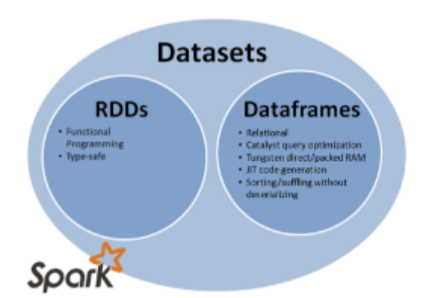
\includegraphics[width=0.3\textwidth]{DfDs.png}\\
  Figure 1: DataSets relation with RDDs and DataFrames (from the slides)
\end{center}

 
 
 \item What will be the result of running the following code on the table people.json, shown below? Explain how each value in the final table is calculated.
 \begin{verbatim}
val people = spark.read.format("json").load("people.json")
val windowSpec = Window.rowsBetween(-1, 1)
val avgAge = avg(col("age")).over(windowSpec)
people.select(col("name"), col("age"), avgAge.alias("avg_age")).show

people.json
{"name":"Michael", "age":15, "id":12}
{"name":"Andy", "age":30, "id":15}
{"name":"Justin", "age":19, "id":20}
{"name":"Andy", "age":12, "id":15}
{"name":"Jim", "age":19, "id":20}
{"name":"Andy", "age":12, "id":10}
 \end{verbatim}
 The result of running the abovementioned code is the following: 
 \begin{center}
  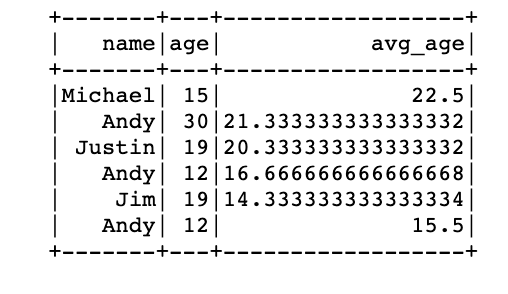
\includegraphics[width=0.5\textwidth]{result.png}\\
  Figure 2: Content of the DataFrame "people"
 \end{center}
Those displayed are the columns selected (name, age, avg\_age). The last one (avg\_age) is filled with values computed on the WindowSpec defined through the rowsBetween method, that includes the frame boundaries (-1,1). Then, the computed result is the average value among the current row age value, the previous row age value (if the previous row exists) and the next row age value (if the next row exists).
 
 \item What is the main difference between the log-based broker systems (such as Kafka), and the other broker systems.\\\\
\noindent The main difference between log-based broker systems and non-log based ones is that the latters don't provide \textbf{durability}, since typically when a message is read, is automatically deleted. \\
Log based brokers aim is to offer a messaging service where producers can append data to a list (log) which consumers can read sequentially. Moreover, the log can be partitioned and distributed in more machines to allow load-balancing. \\Logs are also very important since they facilitate the decoupling between the consumer/producer. For instance, in Kafka, if a producer outputs more information than the consumer can read, the broker stores the messages until the recipient does not receive it.
 
 \item Compare the windowing by processing time and the windowing by event time, and explain how watermarks help streaming processing systems to deal with late events.
 
 Stream processing systems do not require a global view of the input stream to process data in real-time. In fact, they use windowing to partition the data stream, take a fragment of it and do the analysis. \\
 During processing, each data element in the stream needs to be associated with a timestamp, that can recorded following one of the two following  policies:
 \begin{itemize}
\item \textbf{Event time}: the time at which an event actually occurs, so that timestamps are data-dependent and embedded into each record at the source;
\item \textbf{Processing time}: the wall-clock time when the event is received by the streaming application and processed.
 \end{itemize}
 These two alternatives must be taken into account when we choose the Time-based policy to do windowing management: if we window the data by \textit{processing time}, the SPS buffers up incoming data into windows until some fixed amount of processing time has passed (e.g. 5 minutes); while, if we window the data by \textit{event time}, we could have to handle out-of-order events since it reflects the times at which events actually happened. For example, an hourly event time window contains all records that carry an event timestamp that falls into that hour, regardless of the order in which they arrived, or when they are processed.\\\\ Since events can arrive \textit{out of order} and we cannot keep all windows around forever to allow for some lateness in event arrival, the \textbf{watermarks} mechanism has been introduced. Thanks to that, at some point, a window has to be considered done and garbage collected. A watermark is a threshold to specify how long the SPS waits for late events: in particular, it specifies that we assume that all events before \textit{t} have been observed. This is of course a heuristic, as we usually cannot know that for sure (e.g. a watermark that is 5 minutes behind the newest event time seen). Indeed, it is possible that certain elements violate the watermark condition, meaning that even after the Watermark(t) has occurred, more elements with timestamp \textit{t\textquotesingle}  $\leq$\textit{ t} will occur. The SPS can accept these violations, and apply some policies to manage them.
 \item Compare different "delivery guarantees" in stream processing systems.
 
 In Stream processing there are 2 different delivery guarantees:
 \begin{itemize}
     \item Exactly-once delivery, i.e. every message is received only once by all the recipients. The system will not retry additional attempts for re-transmitting events until the streaming application completely recovers. However, to do so, a two-phase commit system must be developed, which is usually not cost-effective for the purpose of the system;
     
    \begin{center}
  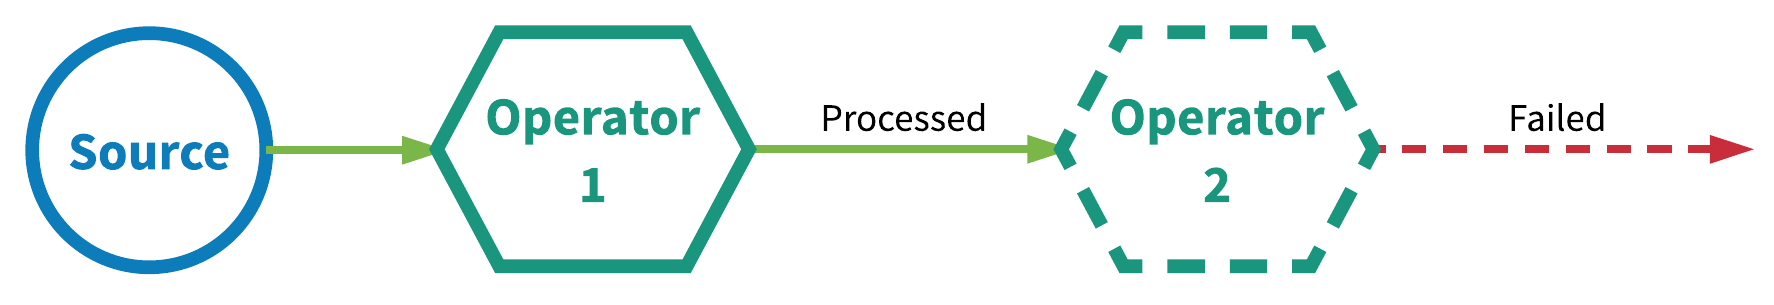
\includegraphics[width=0.5\textwidth]{exactly.png}\\
  Figure 3: https://streaml.io/blog/exactly-once
\end{center}

    \item At-least-once delivery, when a message can be delivered once or more times. In case of a failure, an event can be re-transmitted and some times it is be processed twice. That is the case of Kafka. Kafka normally sends messages only once to every partition in absence of failures. However, in case of crash of a consumer without correct shutdown, it may happen that the consumer process receives the messages twice.
    
    \begin{center}
  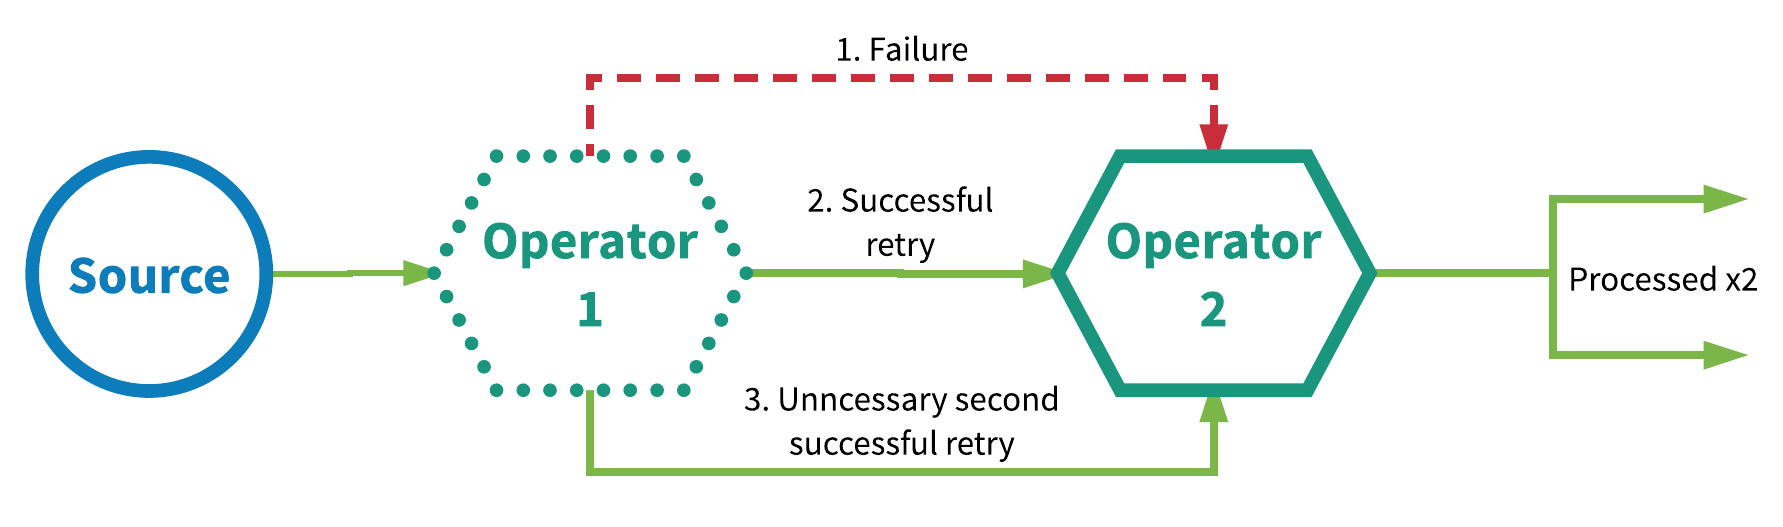
\includegraphics[width=0.5\textwidth]{atleast.png}\\
  Figure 4: https://streaml.io/blog/exactly-once
\end{center}
 \end{itemize}
 For what concerns Kafka delivery guarantees, messages are guaranteed to be received in the same order when produced by a single partition, however, that does not apply when they are delivered by different partitions.
\end{enumerate}


\end{document}